%%%%%%%%%%%%%%%%%%%%% appendix.tex %%%%%%%%%%%%%%%%%%%%%%%%%%%%%%%%%
%
% sample appendix
%
% Use this file as a template for your own input.
%
%%%%%%%%%%%%%%%%%%%%%%%% Springer-Verlag %%%%%%%%%%%%%%%%%%%%%%%%%%

\appendix

\chapter{Code Listing}

On request of the supervisor for this project, program code listing is not included in this document. Instead, the programs can be found on the accompanying DVD and on Github at the following address:\\
\begin{center}
\url{https://github.com/SEDur/IndiEngiSchola}
\end{center}

\chapter{Plots of Time Step Execution Speed for Duration of Simulations}

Below are a series of plots that show the raw time step execution speed for each method and domain size.

\begin{figure}[H]
\centering
  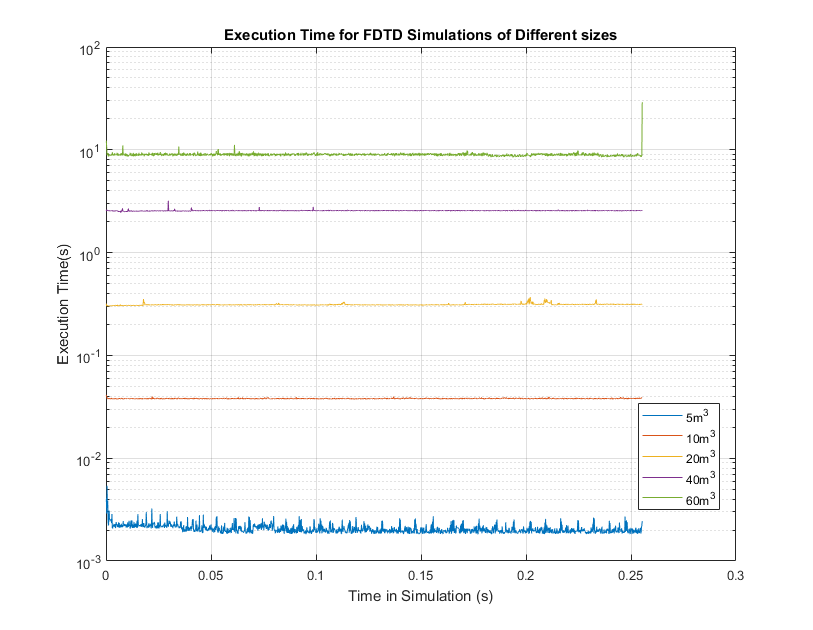
\includegraphics[width=\textwidth]{./graphics/FDTD simulation execution time.png}
  \caption{Execution times for FDTD simulations in domains of increasing size}
\end{figure}

\begin{figure}[H]
\centering
  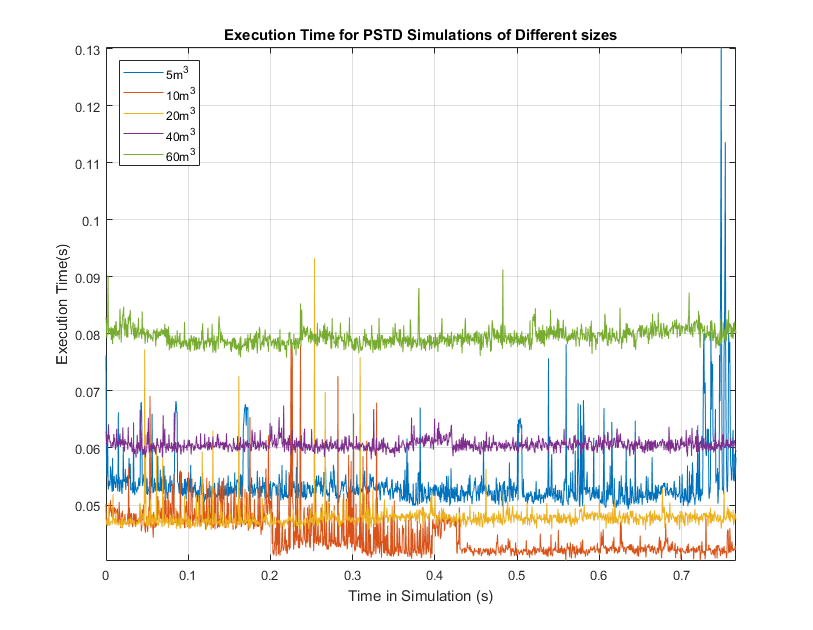
\includegraphics[width=\textwidth]{./graphics/PSTD Simulation Execution Times.png}
  \caption{Execution times for PSTD simulations in domains of increasing size}
\end{figure}

\begin{figure}[H]
\centering
  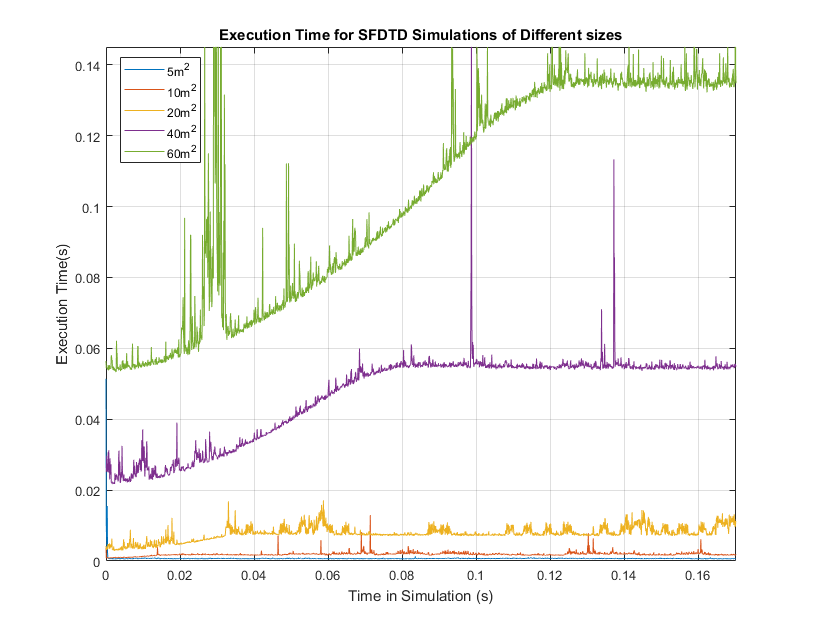
\includegraphics[width=\textwidth]{./graphics/SFDTD simulation execution time.png}
  \caption{Execution times for SFDTD simulations in domains of increasing size}
\end{figure}

The aim of these plots is to better show the stark contrast between each methods execution speed. The PSTD execution speed data shows that execution times are sufficiently low that they are significantly effected by the speed of executing background processes. The FDTD data shows that execution times increase exponentially with venue size, but the time step execution speed is relatively consistent. The SFDTD data shows that the method greatly reduces the execution time early in the simulation, thus reducing the average execution speed of the simulation. As the wavefronts propagate and begin to reflect and diffuse, the execution times of the SFDTD methods appear to stabilise.